\documentclass[11pt,a4paper]{scrartcl}

%%%%%%%%%%%%%%%%%%%% PACKAGES %%%%%%%%%%%%%%%%%%%%%%%%%%

\usepackage[utf8]{inputenc}
\usepackage[T1]{fontenc}
\usepackage[english]{babel}
\usepackage[autostyle]{csquotes}

\usepackage{lmodern}
\usepackage[pdftex]{graphicx}
\usepackage{pdfpages}

\usepackage[noblocks]{authblk}
\usepackage{orcidlink}
\usepackage{wasysym}
\usepackage{fontawesome5}
\usepackage{sty/repostatus}

\usepackage[all]{nowidow}
\usepackage{multicol}
\usepackage{amsmath} % needed for table legend
\usepackage{booktabs} % better looking tables
\usepackage{threeparttable} % needed for better table layouts
\usepackage{hologo} % Provides logos for, e.g., BibTeX

\usepackage[margin=1.5cm, includefoot]{geometry}
\usepackage{fancyhdr}
\pagestyle{fancy}
\fancyhf{}
\renewcommand{\headrulewidth}{0pt}
\rfoot{\thepage}

\usepackage{enumitem}
\setitemize[itemize]{itemsep=0.1em, parsep=0em, topsep=0.2em}
\setitemize[enumerate]{itemsep=0.1em, parsep=0em, topsep=0.2em}

\usepackage{tcolorbox} % used for community feedback hint
%\usepackage{showframe} %% REMOVE BEFORE FINAL RENDERING
\usepackage[colorinlistoftodos,prependcaption]{todonotes} %% REMOVE BEFORE FINAL RENDERING

\usepackage[style=numeric,datamodel=software]{biblatex}
\usepackage{software-biblatex}
\ExecuteBibliographyOptions{
    halid=true,
    swhid=true,
    swlabels=true,
    vcs=true,
    license=true
}
\usepackage[toc,section=section]{glossaries}

\usepackage{hyperref}
\hypersetup{
    pdfauthor={Druskat, S.; Bertuch, O.; Juckeland, G.; Knodel, O.; Schlauch, T.},
    pdfkeywords={Research software; Software publication; Software metadata; Automation; Deposition; Workflows; Repositories; Metadata extraction; Metadata harvesting; Metadata formats; FAIR; FAIR4RS; Provenance; Reproducibility},
    pdflang={EN},
    backref,
    bookmarksopen=true,
    breaklinks=true,
    colorlinks=true,
    linkcolor=blue,
    citecolor=blue
}

%%% Make tables and figures in PDF bookmarks
\usepackage{caption}
\usepackage{bookmark}
\makeatletter
    \pretocmd\endtable{%
      \bookmark[
        rellevel=1,
        keeplevel,
        dest=\@currentHref,
      ]{Table \thetable: \@currentlabelname}%
    }{}{\errmessage{Patching \noexpand\endtable failed}}
    \pretocmd\endfigure{%
      \bookmark[
        rellevel=1,
        keeplevel,
        dest=\@currentHref,
      ]{Figure \thefigure: \@currentlabelname}%
    }{}{\errmessage{Patching \noexpand\endfigure failed}}
    
    \AtBeginDocument{
        \lfoot{\enquote{\@title} \- v\versionnumber}
        
        \hypersetup{
            pdftitle={\@title \- v\versionnumber},
            pdfsubject={\@subtitle: current state of metadata for software and a concept to enhance research software publications with them in an automated fashion}
        }
    }
\makeatother

\usepackage{crossreftools} % used to better control text of namerefs, load after hyperref to let it create linked refs!
\usepackage{subfiles} % Best loaded last in the preamble

\addbibresource{references.bib}

%%%%%%%%%%%%%%%%%%%% METADATA %%%%%%%%%%%%%%%%%%%%%%%%%%

\newcommand*\versionnumber{1}
\newcommand*\version{\\ {\normalsize Version \versionnumber{}}}
\newcommand{\fn}[1]{\texttt{#1}}

%\title{Concept for HERMES}
%\subtitle{Automated workflows for software publication with rich metadata}

\title{Software publications with rich metadata}
\subtitle{State of the art, automated workflows and HERMES concept}

\date{\today \version}

\author[1,*]{Druskat, Stephan \orcidlink{0000-0003-4925-7248}}
\author[2]{Bertuch, Oliver \orcidlink{0000-0002-2702-3419}}
\author[3]{Juckeland, Guido \orcidlink{0000-0002-9935-4428}}
\author[3]{\authorcr Knodel, Oliver \orcidlink{0000-0001-8174-7795}}
\author[1]{Schlauch, Tobias \orcidlink{0000-0001-8760-8913}}
\renewcommand\Affilfont{\footnotesize}
\affil[1]{Deutsches Zentrum für Luft- und Raumfahrt e.\,V.}
\affil[2]{Forschungszentrum Jülich GmbH}
\affil[3]{Helmholtz-Zentrum Dresden-Rossendorf e.\,V.}
\affil[*]{Corresponding Author (\href{mailto:team@software-metadata.pub}{team@software-metadata.pub})}

%%%%%%%%%%%%%%%%%%%% GLOSSARY ENTRIES %%%%%%%%%%%%%%%%%%%%%%%%%%

\makeglossaries
\longnewglossaryentry{ci-cd}
{
    % \label{qo8o3ddicwv8}
    name=CI/CD
}{
    Describes continuous integration/continuous deployment solutions, usually integrated in version control platforms
    to run automated workflows triggered by changes uploaded to the version control service. These workflows are
    primarily used to run automated software tests, but can also be used to run any other software automatically.
    Examples for CI/CD tools include GitLab CI, GitHub Actions and Jenkins automation servers.
}
\longnewglossaryentry{sw-package}{
    %\label{ryblo0s6xdu}
    name=Software Package,
    text=software package
}{
    Describes a unit of functionally and/or semantically self-contained software. This meaning is opposed to the notion
    of package in some programming language, e.g., Java, where it is used to signify the namespace of a smaller unit,
    e.g., a source code file or a class. Other terms for software package include: (software) product, software (sg.),
    piece of software.
}
\longnewglossaryentry{dev-platform}{
    %\label{sr1ngka3xwwa}
    name=Software Development Platform
    text=software development platform
}{
    means an online platform that supports the software development process through the combination of a version-controlled source code repository and additional tools such as issue trackers, code review tools, automation pipelines, etc. Popular examples are GitHub and GitLab.
}
\newglossaryentry{sourcerepo}{
    %\label{sb2fsk1enr1}
    name=Source Code Repository,
    text=source code repository,
    plural=source code repositories,
    description={is a version controlled storage of directories and files usually as part of a software development platform}
}
\newglossaryentry{pubrepo}{
    %\label{bu8qxagwu08b}
    name=Publication Repository,
    text=publication repository,
    plural=publication repositories,
    description={A public catalogue of published artifacts that contains both the artifacts themselves as well as standardized metadata for the artifact. Each artifact is addressable with a unique identifier}
}
\newglossaryentry{repostatus}{
    %\label{msegj6m7qry}
    name=Repository Status Controlled Vocabulary,
    text=repository status,
    plural=repository states,
    description={Based on the terminology from \url{https://www.repostatus.org}, we use the different stati throughout this paper. Stati involve \repostatus[label]{Concept}, \repostatus[label]{WIP}, \repostatus[label]{Suspended}, \repostatus[label]{Abandoned}, \repostatus[label]{Active}, \repostatus[label]{Inactive}, \repostatus[label]{Unsupported} and \repostatus[label]{Moved}}
}
\newglossaryentry{webhook}{
    name=Webhook,
    text=webhook,
    plural=webhooks,
    description={Common web technique: some software sending an HTTP POST request to a target system with the intent to trigger some kind of reaction. The request may carry a (JSON) payload, containing context, authentication, parameters and other information}
}
\newglossaryentry{static-metadata}{
    name=Statically available metadata,
    text=statically available metadata,
    plural=statically available metadata,
    description={Statically available software metadata can be accessed from static sources such as dedicated files or parts of files, version control systems or other forms of repositories, \gls{ci-cd} contexts, file systems or platform APIs}
}


% This definition is not perfect - it's missing edge cases like runtimes influenced by random, by time, by environment (language/timezone/...)
% \newglossaryentry{runtime-metadata}{
%     name=Runtime-specific metadata,
%     text=runtime-specific metadata,
%     plural=runtime-specific metadata,
%     description={Runtime-specific metadata is aggregated for software at specific runtimes and not \glslink{static-metadata}{statically available}. Examples include benchmarking results, statistics relating to call graphs, availability metrics, throughput metrics, etc. Secondary runtime-specific metadata includes metrics that are aggregated at runtime, but may be available statically}
% }

%%%%%%%%%%%%%%%%%%%% DOCUMENT %%%%%%%%%%%%%%%%%%%%%%%%%%

\begin{document}
\maketitle
\thispagestyle{empty}

\begin{abstract}\label{abstract}
\addsec{Abstract}
To satisfy the principles of FAIR software, software sustainability and software citation, research software must be formally published.
Publication repositories make this possible and provide published software versions with unique and persistent identifiers.
However, software publication is still a tedious, mostly manual process.

To streamline software publication, HERMES, a project funded by the Helmholtz Metadata Collaboration, develops automated
workflows to publish research software with rich metadata.

The tooling developed by the project utilizes continuous integration solutions to retrieve, collate, and process existing metadata
in source repositories, and publish them on publication repositories, including checks against existing metadata requirements.
To accompany the tooling and enable researchers to easily reuse it, the project also provides comprehensive documentation and
templates for widely used CI solutions. In this paper, we outline the concept for these workflows, and describe how our solution
advance the state of the art in research software publication.
\end{abstract}

\vspace*{\fill}
\begin{center}
    \footnotesize
    This work is licensed under \href{https://creativecommons.org/licenses/by/4.0/}{\faCreativeCommons\faCreativeCommonsBy\,4.0}.    
\end{center}
\clearpage



\begin{tcolorbox}[colback=blue!5!white,colframe=blue!75!black,title=Requesting community feedback]
\paragraph{Community feedback}\label{community-feedback}

At this stage, we would like to reach out to the community to gain insights into what desirable solutions can 
look like, what potential pitfalls are, etc.

We kindly ask readers and other interested parties to provide feedback on the concept detailed here via its PubPeer page at
\url{https://software-metadata.pub/concept-paper-community-reviews}.
\tcblower

\begin{itemize}  
    \item What metadata types, formats and standards are missing from our lists in \nameref{subsec:metadata}?
    \item Does table \ref{tab:comparision-metadata-types}, mapping metadata types to metadata formats, miss anything important, or misrepresent something?
    \item Does table \ref{tab:workflows} miss any other publication workflows you know and should be included?
    \item What are desired additional outputs of the automated workflows in addition to deposition in the targeted
          publication repositories? E.g., would the creation of \nameref{par:metadata-formats-codemeta} or 
          \nameref{par:metadata-formats-cff} be helpful, are there other desired output types?
    \item Should the HERMES pipelines leverage workflow domain specific languages (such as
          \href{https://www.commonwl.org/}{Common Workflow Language (CWL)}, \href{https://nextflow.io/}{Nextflow}, etc.)
          to knit together existing tools, such as harvesters (e.g., \nameref{par:tooling-somef}), 
          converters (e.g., \nameref{par:tooling-cffconvert}), and deposition tools (e.g., \nameref{par:workflows-zenodraft})?
    \item While we initially restrict the scope of HERMES with regard to metadata validation to linting 
          (see \ref{subsec:concept-scope}), there may be other factors that influence the validity of metadata.
          It is known that VCS contributors metadata, for example, is unsuitable to be used as valid authorship
          metadata, as there may be people qualifying as authors who have not contributed to a source code repository,
          or people that are contributors but do not qualify as authors under a given definition of authorship.
          Therefore, other metadata sources, such as files in the Citation File Format may be more trustworthy.
          What are other pitfalls concerning the validity of metadata that HERMES should be aware of?
\end{itemize}

\end{tcolorbox}
\clearpage


\section{Introduction}\label{sec:introduction}
There is increasing awareness that software is a valid research output and should be treated as such~\cite{jaySoftwareMustBe2021,SoftCitePrinciples}. Thus, software is increasingly published in public repositories or software journals~\cite{TrackingCitations}. This is a necessary step in transferring the FAIR principles to software~\cite{FAIR4RS-Principles} -- i.e., for finding, understanding, reusing, sharing and citing software -- and promoting it to first class research citizenship. Recent policy updates from universities, research institutes (e.g., at Helmholtz Association (HGF)~\cite{HelmholtzSWPolicy}) and funders such as the Deutsche Forschungsgemeinschaft (DFG)~\cite{DFG-GRP19} reflect this progress. Metrics for published software may inform funding decisions in the future.

The main driver for a fulfillment of the functions of FAIR software is software metadata~\cite{FAIR4RS-FreshLook}, and thus, publication of research software with rich metadata is essential. In modern research software development, metadata on different software properties is created automatically, semi-automatically or manually at different stages, and in different places and formats. While this metadata can already be collected, verified and validated, and edited to be published with software, there is currently no streamlined, automated process or workflow to do so. This in turn disincentivizes the researchers, research software engineers and maintainers who create and maintain research software, to publish it with rich metadata.

In this paper, we describe a concept for automated publication of research software with rich metadata via existing automation tools. The concept is being developed in the project HERMES (\textbf{HE}lmholtz \textbf{R}ich \textbf{ME}tadata \textbf{S}oftware Publication), conducted at the German Aerospace Center (DLR), Forschungszentrum Jülich (FZJ) and Helmholtz Zentrum Dresden Rossendorf (HZDR), and funded by the Helmholtz Association of German Research Centers‘ Helmholtz Metadata Collaboration (HMC) initiative (see \nameref{acknowledgments}).

The work packages related to the concept as described in this document yield a number of outputs: 

\begin{itemize}
  \item \textbf{software} to retrieve existing software metadata in source code repositories, collate and process them to produce a coherent set of metadata for the current state of a given repository;
  \item \textbf{templates}, e.g. for \gls{ci-cd} systems and workflow engines, to run the metadata tools on a users' source repositories;
  \item \textbf{documentation} and examples for the outputs the project provides.
\end{itemize}

In the following sections, we describe the state of the art for software metadata, available tooling to work with metadata and existing approaches to automation. We then lay out our concept for research software deposits with rich metadata in automated workflows for two target platforms. In the process, we specify requirements for the structure and contents of source code repositories, define an iterative process for the inclusion of increasingly unstructured metadata, detail the scope of the project and provide a high-level outline of the implementation of both interfaces and tooling. 

% In a version 2 of this paper, we need to overhaul this paragraph - especially the part on that we rely/base on feedback
We request community feedback for the concept detailed here (see \crtlnameref{community-feedback} above). Based on feedback we receive, the HERMES project partners design interfaces and develop software tools to automatically aggregate metadata included in software repositories. The interfaces and software tools combination provide an extensible, \gls{ci-cd}-driven serverless solution that enables direct ingestion into publication repositories, such as Zenodo or Harvard Dataverse, and other repositories using the underlying \nameref{par:repos-inveniordm} or \nameref{par:repos-dataverse} software. 



\clearpage
\section{State of the art}\label{sec:state-of-the-art}




\subsection{Metadata}\label{subsec:metadata}
Software metadata provides information about software, or specific properties of software. It is created intentionally, or generated as a side-product during software development processes. As such, metadata can also pertain to different parts of software, or a \gls{sw-package} as a whole. Additionally, it can exist in different modes, i.e., as structured or unstructured metadata. It may also pertain to different aspects of the software, e.g., the license regulating its use and development, its creation context, etc. Consequently, there exist different types of metadata.

Software metadata may be provided in dedicated files, or as part of some file. Metadata can also be part of version control systems
or other forms of repositories, as well as the file system or platform hosting the source code. We define these as \gls{static-metadata}.

Structured metadata, especially when persisted in files, may furthermore come in specific formats. These may be standard formats through formal processes or community practice.

In this section, we describe different types of software metadata, as well as formats they are provided in. Table \ref{tab:comparision-metadata-types} on page \pageref{tab:comparision-metadata-types} shows a mapping of metadata types to the formats they are commonly provided in, based on our experience.




\subsubsection{Types}\label{subsubsec:metadata-types}
There are generic types of metadata that exist for software but may also be found for other digital data, as well as software-specific metadata.
The latter is partly due to the fact, as described in \cite{PeerJSoftVsDataCitation}, that software is both static (as source code, i.e., digital data)
and dynamic (at runtime).

% \newcommand*\static{\item[$\bullet$]}
% \newcommand*\dynamic{\item[$\circ$]}

\begin{multicols}{2}
    \raggedright
    Generic software metadata includes:
    \begin{itemize}  
        \item Software name
        \item File system metadata \\ {\small (e.g., file sizes, number of files, etc.)}
        \item Authorship and contributorship information
        \item Reference to the documentation pertaining to the software
        \item Legal and licensing information
        \item Funding information
        \item Domain context
        \item Citation metrics
        \item Location metadata \\ {\small (e.g., download or instance URLs, etc.)}
        \item Publication dates, etc.
        \item Categorization information \\ {\small (e.g., application category, keywords, etc.)}
        \item Availability information \\ {\small (e.g., purchasing costs, etc.)}
        \item Identifiers
        \item Relational metadata \\ {\small (e.g., software \textit{is part of} another work)}
        \item High-level description
    \end{itemize}
    \columnbreak
    
    Software-specific metadata includes:
    \begin{itemize}  
        \item Dependency information
        \item Lines of code
        \item Programming language
        \item Version information \\ {\small (e.g., metadata from version control systems, publication platforms, or even file names; version identifiers, etc.)}
        \item Runtime requirements, including hardware requirements
        \item References to work the software is built on, or relates to
        \item Software metrics \\ {\small (e.g., quality metrics like code coverage, ...)}
        \item Development metrics \\ {\small (e.g., pertaining to issues, pull requests, ...)}
        \item Usage metrics \\ {\small (e.g., downloads, stars, citations, ...)}
        \item Infrastructural metadata \\ {\small (e.g., build and CI systems used to produce version artifacts, etc.)}
    \end{itemize}
\end{multicols}





\subsubsection{Formats}\label{subsubsec:metadata-formats}
Some metadata are persisted in files that have specific formats, or are integrated in specific formats as part of other files.
Such files are usually persisted and version controlled alongside source code. 

Other metadata must be retrieved from third-party systems, e.g., the version control system, source code platform
(GitHub, GitLab, or other), etc., if available. Some are only available on other platforms or systems and may not be
retrievable from the source code repository.

\paragraph{Plain text files}\label{par:metadata-formats-plaintext}
Some software metadata is provided in plain text. There are some typical dedicated plain text files, such as license files
(\fn{LICENSE}, \href{https://reuse.software/spec/}{REUSE Specification} compliant files, etc.) or
citation metadata files (plain text \fn{CITATION} files), that can reasonably be assumed to contain only relevant metadata. 

Other files mix metadata and other information, such as documentation files (\fn{README} files and other plain text documentation),
community files containing contributor information, a code of conduct, governance information, or other information.
Other relevant metadata may be provided in plain text in a less overt manner, e.g., embedded in source code files. 

Generally, while plain text metadata is easily accessible for human readers, they are perhaps the hardest to process using
automated approaches. This is due to their less structured form and a lack of clarity with regard to semantics. A plain 
\fn{CITATION} file, for example, may provide retrievable publication metadata, but there is no way of automatically verifying
that the metadata unambiguously pertains to a specific version of the software it is provided with, or indeed something
else entirely. 

The same is true for any plain text metadata and specifically for metadata that are embedded in plain text: while methods
exist to extract metadata from plain text, they rely on heuristics that can only produce assumptions with some degree of
confidence in their significance and correct categorization.

\paragraph{schema.org files}\label{par:metadata-formats-schema-org}
schema.org~\cite{SchemaOrg} provides schemas for structured data markup. These are commonly used in HTML to provide metadata that is reused by search engines. schema.org schemas are also used as basis for metadata in RO-Crate~\cite{RO-Crate}. Additionally, there is ongoing work\footnote{\url{https://github.com/codemeta/codemeta/issues/232}} to add missing terms from the CodeMeta schema~\cite{CodeMetaSchema} to schema.org.

\paragraph{CodeMeta files}\label{par:metadata-formats-codemeta}
CodeMeta~\cite{CodeMetaSchema} is a format for generic software metadata, implemented in JSON-LD, extending \nameref{par:metadata-formats-schema-org}. It is used to provide comprehensive information about software, with some focus on academic use cases.

\paragraph{Citation File Format}\label{par:metadata-formats-cff}
The Citation File Format~\cite{CffSchema} is a format to provide citation metadata for software, implemented in YAML. Its focus is exclusively to provide citation-relevant metadata in a form that is both human- and machine-readable.

\paragraph{Zenodo JSON files}\label{par:metadata-formats-zenodo-json}
The open access publication platform Zenodo~\cite{Zenodo} uses its own metadata schema, implemented in JSON\footnote{\url{https://developers.zenodo.org/\#github}}. The schema is used in practice to provide metadata for works that are being published on Zenodo, e.g., through the GitHub-Zenodo integration (see also \nameref{par:workflows-pull} and table \ref{tab:workflows} on page \pageref{tab:workflows}).

\paragraph{\hologo{BibTeX} files}\label{par:metadata-formats-bibtex}
\hologo{BibTeX} files contain citation metadata for one or more works. The format is standardly used as input for citations and bibliographies
in \LaTeX\ documents, but is sometimes also adapted to provide convenient citation metadata for software, for example in a dedicated file in
\glspl{sourcerepo} (sometimes called \fn{CITATION}), or embedded in a text or marked up document such as a \fn{README} file. 

In the context of metadata retrieval, \hologo{BibTeX} files or snippets pose the same challenges as plain text due to their generic nature.
It is hard to understand if a \hologo{BibTeX} item is describing the software package it is provided with, one of its versions, or something
else entirely. The biblatex-software~\cite{sw:biblatex-software} package for \LaTeX\ solves issues around citing different software reference
types in scholarly publications, but the general issue with \hologo{BibTeX} items and their relation to given software remains.

\paragraph{Manifest files}\label{par:metadata-formats-manifests}
Manifest files describe a \gls{sw-package} or a subunit of a software package. They exist for different programming languages and frameworks and come in a variety of implementation formats. Some examples include Project Object Model (POM) XML files for Java projects using the Apache Maven build management tool, JAR manifests for packaged Java applications, or \fn{setup.py}/\fn{pyproject.toml} files that contain metadata for Python packages built with Python’s distutils.

\paragraph{Configuration files}\label{par:metadata-formats-config}
Configuration files are often added to source code repositories to leverage third-party tools such as \gls{ci-cd} services or source code or documentation generators. They come in different formats, of which common ones are plaintext key-value definitions, INI, TOML, YAML, JSON and XML. Configuration files may include metadata pertaining to, e.g., software dependencies, development and publication processes, etc. One popular example for configuration files that contain contribution metadata are those for the All Contributors\footnote{\url{https://allcontributors.org}} specification.

\paragraph{Linked Data files}\label{par:metadata-formats-linked-data}
Linked data provides an extensible way to describe research software in depth. Common linked data formats are based on RDF~\cite{W3C-RDF}, using serializations like JSON-LD~\cite{W3C-JSON-LD} or Turtle~\cite{W3C-RDF-Turtle}. They express not just attributes or simple relations, but reuse formalized concepts (ontologies) to describe usage, ideas, context, etc., in much greater depth than other formats listed above.

Although ontologies are a powerful concept, there does not seem to be sufficient uptake of using software ontologies to describe software in practice. This may change in the future.

Commonly known ontologies for software include Software Description Ontology~\cite{SoftDescOnto}, Software Ontology~\cite{SoftwareOntology}, SEON~\cite{SeonOntology} and DOAP~\cite{DoapOntology}.

\paragraph{Version control system}\label{par:metadata-formats-vcs}
The version control system in use may provide valuable metadata from the commit history. Especially in distributed version control systems like Git, 
the complete history is available locally. These metadata are part of a project context and not formalized in a file, but may be retrieved by using command
line interfaces or wrapping libraries of the version control system at hand. They may provide insights for example into contributors, file metadata,
changes over time or related software/data.

\paragraph{Platform API responses}\label{par:metadata-formats-apis}
While not strictly a format, software metadata is also available from different (e.g., REST, GraphQL) APIs, such as those for querying software
development platforms (like GitHub or GitLab), WikiData, or publication repositories. These may provide metadata on software development
processes, version control, contributions, publications, as well as other metadata. These APIs can usually be queried through their
endpoints -- or globally using a common query language such as~\cite{W3C-SPARQL} -- and responses are usually provided as JSON or XML
that can easily be persisted and reused.




\subsection{Standards}\label{subsec:metadata-standards}
As of now, there are no software metadata formats relating to our work that are formally standardized and cover HERMES’
scope completely. Some de facto standards exist:

\begin{itemize}
    \item CodeMeta’s ongoing integration\footnote{\url{https://github.com/codemeta/codemeta/issues/232}} into schema.org
          promises at least future de facto standardization. 
    \item The DataCite Metadata Schema~\cite{DataCiteSchema}, although used widely, has a much more generic scope again
          than, e.g., CodeMeta, and does not implement as large a vocabulary pertaining to software 
          (see the CodeMeta-DataCite crosswalk\footnote{\url{https://codemeta.github.io/crosswalk/datacite/}}).
\end{itemize}

Standards in similar stages exist in related areas, such as for research objects in general: 
\begin{itemize}
    \item RO-Crate~\cite{RO-Crate} packages research objects with their metadata, its schema based on schema.org.
    \item BagIt~\cite{BagItRFC} is a generic packaging standard used in, e.g., libraries, to package file structures with
          metadata, where the metadata schema is very generic and not targeted to software specifically.
\end{itemize}




\subsection{Integrations}\label{subsec:metadata-integrations}
Some platforms and tools provide integrations for some of the above-mentioned formats. As opposed to concrete (software)
tools for working with formats that are available to end-users, integrations are embedded in their hosts and are not
directly addressable by users.

\paragraph{Plain text}\label{par:metadata-integrations-plaintext}
Many platforms support metadata provided in plain text or light\-weight markup languages by rendering them for presentation
to end users. This often includes detecting URLs and converting them to HTML hyperlinks. Examples include Markdown
rendering on, e.g., GitHub, GitLab, and many other platforms.

\paragraph{schema.org}\label{par:metadata-integrations-schemaorg}  
RO-Crate~\cite{RO-Crate} uses schema.org~\cite{SchemaOrg} schemas to record and provide core metadata. Both \nameref{par:repos-dataverse} and
\nameref{par:repos-inveniordm} offer metadata exports as schema.org JSON-LD.

\paragraph{CodeMeta}\label{par:metadata-integrations-codemeta}
Software Heritage~\cite{SWHArchive} uses a subset\footnote{\url{https://docs.softwareheritage.org/devel/swh-indexer/metadata-workflow.html\#supported-codemeta-terms}}
of the CodeMeta vocabulary to map intrinsic metadata formats discovered in source repositories.
CaltechDATA ingests CodeMeta files to create metadata records from the included metadata~\cite{ASCL-CaltechAMES}~\cite{sw:AMES}.
The Astrophysics Source Code Library (ASCL) produces pre-filled Code\-Meta files from its records~\cite{ASCL-Software-Citation} --
this functionality is accessible to users through appending the URL for a record page with \fn{/codemeta.json}.

\paragraph{Citation File Format}\label{par:metadata-integrations-cff}
\begin{itemize}  
    \item Via its Github-Zenodo integration, Zenodo ingests the metadata from \fn{CITATION.cff} files and uses them to populate their
          metadata records~\cite{sw:invenio-github} (see also table \ref{tab:workflows} on page \pageref{tab:workflows}).
    \item Via its connector browser plugins, Zotero ingests \fn{CITATION.cff} files discovered in source code repositories and saves
          the metadata in its internal format~\cite{FennerBlogCff}.
    \item JabRef can import \fn{CITATION.cff} files (feature merged, currently awaiting release\footnote{\url{https://github.com/JabRef/jabref/issues/7945}}).
    \item The Astrophysics Source Code Library (ASCL) produces pre-filled \fn{CITATION.cff} files from its records. This functionality
          is accessible to users through appending the URL for a record page with \fn{/CITATION.cff}~\cite{ASCL-Software-Citation}.
    \item GitHub provides a template\footnote{\url{https://docs.github.com/en/repositories/managing-your-repositorys-settings-and-features/customizing-your-repository/about-citation-files}}
          for creating new \fn{CITATION.cff} files via its UI and ingests existing \fn{CITATION.cff} files, extracts the metadata, converts
          them to a citation style and BibTeX, and provides them in a widget for end users to copy~\cite{FennerBlogCff}. 
          There is a feature request to implement the same for GitLab\footnote{\url{https://gitlab.com/gitlab-org/gitlab/-/issues/337368}}.
    \item An extension\footnote{\url{https://www.higithub.com/citation-file-format/issue/citation-file-format/356}} to the Sphinx platform 
          for documentation rendering ingests an existing \fn{CITATION.cff} file and, converts it to different citation formats, and provides 
          it to end users in a widget for copying (see example in~\cite{CffSphinxExample}).
    \item Software Heritage can ingest \fn{CITATION.cff} as intrinsic metadata format and map it
          (see \href{https://docs.softwareheritage.org/devel/swh-indexer/metadata-workflow.html}{SWH Indexer Metadata Workflow},
          referenced in~\cite{FennerBlogCff}).
\end{itemize}

\paragraph{Zenodo JSON}\label{par:metadata-integrations-zenodo-json}
Via its GitHub-Zenodo integration, Zenodo ingests\footnote{\url{https://developers.zenodo.org/\#add-metadata-to-your-github-repository-release}}
\fn{.zenodo.json} files and populates metadata records from the provided metadata~\cite{sw:invenio-github}.

\paragraph{BibTeX}\label{par:metadata-integrations-bibtex} 
Usually, the metadata from \hologo{BibTeX} \fn{.bib} files are converted into string formatted in a citation style and displayed 
as citations and items in the references list of \LaTeX\ based documents.

biblatex-software~\cite{sw:biblatex-software} is a reference biblatex implementation of a bibliography style extension
that includes software-specific \hologo{BibTeX} entries and integrates these metadata in \LaTeX\ documents.

\paragraph{Manifest files}\label{par:metadata-integrations-manifests}
Some or all information from manifest files is rendered on package/artifact repositories’ sites for the respective package,
e.g., on \href{https://mvnrepository.com}{Maven Central}, \href{https://pypi.org}{PyPI}, 
\href{https://www.npmjs.com}{NPMJS}, \href{https://www.debian.org/distrib/packages}{Debian Packages} etc. 



\subsection{Tooling}\label{sec:tooling}
The following section is an attempt to gather tools available for metadata extraction, collection and durable publication.
Please note: section \ref{subsubsec:workflows-blocks} contains any tooling to be used as building blocks
for (automatable) workflows around software depositions. These lists may not necessarily be complete.

\subsubsection{Metadata}\label{subsec:tooling-metadata}
Existing toolsets for metadata may operate on different stages of metadata presence. The spectrum starts at zero 
prior information and requires extraction from arbitrary text files and context information. Moreover, it can be 
accomplished by reusing software package metadata via so called crosswalks, or even  conversions between different
metadata formats. Some may give users a hand to create well-structured metadata from the start.

\paragraph{Software Metadata Extraction Framework (SoMEF)}\label{par:tooling-somef}
SoMEF~\cite{sw:SoMEF}~\cite{SoMEF} extracts data from \fn{README} text files and
other files that may include metadata using a neural network. It may also retrieve details from \gls{dev-platform}
such as GitHub, using their APIs. It creates, e.g., CodeMeta JSON-LD or Turtle RDF files using 
The Software Ontology~\cite{SoftDescOnto}. The projects \gls{repostatus} is \repostatus[label]{active}.

\paragraph{CaltechDATA Automated Metadata Service (AMES)}\label{par:tooling-ames}
AMES~\cite{sw:AMES} may be used to create and update scholarly output records in services like
CaltechDATA, highly specific for Caltech and based on \ref{par:repos-inveniordm}. For software publications
a Python script to update \nameref{par:repos-inveniordm} records from \nameref{par:metadata-formats-codemeta}
files is in use~\cite{ASCL-CaltechAMES}. The projects \gls{repostatus} is \repostatus[label]{active}.

\paragraph{codemeta2cff GitHub Action}\label{par:tooling-codemeta2cff}
The codemeta2cff GitHub Action~\cite{sw:codemeta2cff} provides automatic conversion from a
\nameref{par:metadata-formats-codemeta} file to a \nameref{par:metadata-formats-cff} file in a GitHub Action.
The projects \gls{repostatus} is \repostatus[label]{suspended}.

\paragraph{CodeMeta Crosswalks}\label{par:tooling-crosswalks}
CodeMeta Crosswalks~\cite{sw:codemeta-crosswalks} are a set of comma-separated value (CSV) files, containing
two columns. Each row depicts a metadata field in \nameref{par:metadata-formats-codemeta} and a
corresponding field in some other schema. 
While not an executable tool, these crosswalks describe a mapping with limited interoperability, as most
other standards aren’t as detailed.
The projects \gls{repostatus} is \repostatus[label]{inactive}.

\paragraph{CodeMeta Generator}\label{par:tooling-codemeta-gen}
CodeMeta Generator~\cite{sw:codemeta-generator} is a Javascript-based web UI to help you create 
\nameref{par:metadata-formats-codemeta} for inclusion in your software repository. The projects
\gls{repostatus} is \repostatus[label]{inactive}.

\paragraph{Citation File Format Converter}\label{par:tooling-cffconvert}
cffconvert~\cite{sw:cffconvert} is a Python based command line tool to transform a given 
\nameref{par:metadata-formats-cff} file into other destination formats like \nameref{par:metadata-formats-bibtex},
\nameref{par:metadata-formats-codemeta} and others. It is also available as a GitHub Action.
The projects \gls{repostatus} is \repostatus[label]{active}.

\paragraph{Citation File Format Initializer}\label{par:tooling-cffinit}
cffinit~\cite{sw:cffinit} is a Javascript based interactive web form to assist you in creating a 
new or updating an existing \nameref{par:metadata-formats-cff} file in your browser.
The projects \gls{repostatus} is \repostatus[label]{active}.



\subsubsection{Publication repositories}\label{subsubsec:repositories}
\Glspl{pubrepo} are public catalogue containing publications of digital artifacts together with the metadata describing them.
Usually, publication repositories provide landing pages for each artifact, including versions of the same object.
As such, they are different from registries, that usually focus on the collection of metadata and their presentation.
They are also different from archives, that focus on long-term archival of artifacts only. Additionally there may exist
differences in how records are added to publication repositories, registries and archives.

One of the main advantages of publication repositories is that they enable a combination of discovery of digital objects
through their metadata, and direct access to the object artifacts themselves. HERMES focuses on publication repositories
exclusively, and specifically on two publication repository software projects as deposition targets, for the reason that
they represent commonly used platforms both within the Helmholtz Association and beyond: Dataverse project and InvenioRDM.

Research software is also represented in digital preservation archives (like the Software Heritage Archive~\cite{SWHArchive}),
catalogues and directories (like the Research Software Directory~\cite{RSD-2018}). Targeting these platforms may be a 
future direction of development for HERMES, see also \ref{subsubsec:concept-scope-future}.

\paragraph{Dataverse project}\label{par:repos-dataverse}
The \href{https://dataverse.org}{Dataverse project} is an open source repository software.

Its focus is currently on providing services for \href{http://purl.org/dc/dcmitype/Dataset}{Dataset} deposition, although 
software may be deposited as part of datasets, too. No built-in support for software metadata schemas, software licenses
or propagating software metadata to PID registrars is available.

Despite versioning support for datasets, neither integrating software release versioning is available nor support for
software citations as a concept and individual releases.

The Dataverse community runs a working group for software, workflow and container related topics.
Its website can be found at \url{https://swc.wgs.gdcc.io} The projects \gls{repostatus} is \repostatus[label]{active}.

\paragraph{InvenioRDM}\label{par:repos-inveniordm}
The \href{https://inveniosoftware.org/products/rdm/}{InvenioRDM project} has the goal to provide a turn-key research data
management repository based on Invenio Framework and Zenodo. The publication of special software datasets is possible,
but the standard set of metadata for the description of Invenio records is used as well as in \ref{par:metadata-formats-zenodo-json}.

Invenio provides versioning, DOI registration and supports multiple data types for the publication such as Publication, Poster,
Presentation, Dataset, Image, Video/Audio, Software, Lesson, Physical objects or Other 
(list\footnote{See \texttt{upload\_type} at \url{https://zenodo.org/schemas/deposits/records/legacyrecord.json}} taken from Zenodo).
No builtin support for software metadata schemas is available at the moment. 

For a software publication the use of optional webhooks can be used as introduced in \nameref{par:workflows-pull}.

The projects \gls{repostatus} is \repostatus[label]{active}.




\subsection{Workflows}\label{subsec:workflows}
Depositing scientific software to archives like Software Heritage~\cite{SWHArchive} or \crtlnameref{subsubsec:repositories}
requires some kind of workflow, involving manual steps or automation.

Workflows may be coarsely categorized into \enquote{push} or \enquote{pull} based approaches. Both have their pros 
and cons, but within the context of scholarly software publications, push-based approaches have the advantage of 
not having to expose the \gls{sourcerepo} to the publishing service. As making a software FAIR does not require 
code access~\cite{FAIR4RS-Principles}\cite{FAIR4RS-FreshLook}, this may be beneficial to increase the number of 
software publications even for closed source research software.

Table \ref{tab:workflows} on page \pageref{tab:workflows} provides an in-depth overview of known full-fledged workflows
and tools used within custom automated jobs pertaining to software publications. Both categories of workflows are
covered and analysed for their metadata extraction and publication capabilities. Please note: neither the table nor
the following list of building blocks need to be complete.


\paragraph{Pull-based workflows}\label{par:workflows-pull} may be subdivided into \enquote{harvesting} and \enquote{triggered} types.

\enquote{Harvesting} for new or changed datasets is an often used pattern within the world of text and data publications.
The well-known OAI-PMH is used for inter-repository talk, while harvesting in the context of workflows is attached
to pulling commits from public accessible \glspl{sourcerepo}. Retrievals may be scheduled or kicked off by some event.
To provide an example: both the Software Heritage Archive~\cite{SWHArchive} and the Research Software Directory~\cite{RSD-2018}
use scheduled harvesting: they check for changes in source code repositories, publishing repositories, etc. and incorporate them, which 
might involve updating existing metadata.

Using a \gls{webhook} to \enquote{trigger} some action is a well known technique in distributed systems. 
Within the publication business a webhook may even trigger a harvesting action with certain parameters like a target.
The GitHub-Zenodo integration\footnote{\url{https://guides.github.com/activities/citable-code}} is a good example for this,
sending a webhook request on \gls{sw-package} releases (tagged revisions within a \gls{sourcerepo}) to trigger the harvest.

\paragraph{Push-based workflows}\label{par:workflows-push}
While pull-based workflows have their advantages, in some scenarios you might want to publish your software in a more active fashion.

Push-based workflows gather metadata and/or artifacts and deposit them via some API endpoint into a service like a repository,
registry or archive. They may also split certain tasks across different services, which may be harder to achieve with
common pull-based workflows.

Examples for push-based workflows are even harder to find than pull-based workflow approaches. This might be due to the
convenience of commonly known pull-based workflows and the not-yet popular task of software publications. Please let us
know of any prototypical example we haven’t listed in table \ref{tab:workflows} on page \pageref{tab:workflows} yet.


\subsubsection*{Building Blocks}\label{subsubsec:workflows-blocks}
The following tools provide building blocks to create an automatable depositing workflow, interfacing with target repositories, registries or archives.

\paragraph{Zenodraft}\label{par:workflows-zenodraft}
Zenodraft~\cite{sw:zenodraft} and the corresponding GitHub action~\cite{sw:zenodraft-action} may be used to draft, push and publish
new deposits on \href{https://zenodo.org}{Zenodo}, a commonly known general purpose repository based on \nameref{par:repos-inveniordm}.
New and existing deposits may be enhanced with metadata via \nameref{par:metadata-formats-zenodo-json}.
The project's \gls{repostatus} is \repostatus[label]{suspended}.

\paragraph{Software Heritage Github Action}\label{par:workflows-swh-gh-action}
SWH Github Action~\cite{sw:swh-save-action} acts like a webhook: it sends a archive request to an Software Heritage Archive 
API endpoint with the repository to archive given as parameter.
Software Heritage Archive services take care\footnote{See \url{https://docs.softwareheritage.org/devel/swh-indexer/metadata-workflow.html}}
of reading a \nameref{par:metadata-formats-codemeta}, \nameref{par:metadata-formats-cff} or other metadata files via 
\nameref{par:tooling-crosswalks} (if included) to add metadata to its archive.
The project's \gls{repostatus} is \repostatus[label]{suspended}.

\paragraph{Software Heritage Deposit Command Line Tool}\label{par:workflows-swh-deposit-cli}
The CLI part of a SWORD~\cite{SWORD} based deposition service~\cite{sw:swh-deposit-cli} 
for the Software Heritage Archive may be used to actively push metadata and/or artifact ingests.
It seems not to be intended for public usage but integrations with software/data repositories.
The project's \gls{repostatus} is \repostatus[label]{active}.

\paragraph{Dataverse Uploader GitHub Action}\label{par:workflows-dataverse-action}
The Dataverse Uploader Github Action~\cite{sw:dataverse-uploader-action} enables uploading content from a \gls{sourcerepo} into
a \enquote{dataset} on a target \nameref{par:repos-dataverse} installation. It allows to replace all or add to files and their metadata.
The action may also publish a new dataset version afterwards. The projects \gls{repostatus} is \repostatus[label]{active}.





\clearpage
\section{Concept}\label{sec:concept}

\subsection{Overview}\label{subsec:concept-overview}
The coupling of software development platforms with publication repositories for automated data exchange is a first and important step
for easier and automated software publications. This technical foundation also immediately raises the question as to the requirements
towards a source code repository on a development platform to benefit from such automation. Current first generation tools simply copy
the content of a source code repository to create or update a publication repository entry. The metadata of the publication repository
entry can originate from a special file in the source code repository.

Questions addressed by HERMES that extend the status quo are:

\begin{itemize}  
    \item How to automate collation of metadata from different sources for automated publication?
    \item How to treat different components in a source code repository (software, documentation and data)?
    \item How to deal with source code repositories that contain more than one software product?
    \item How to deal with publication of executable software artifacts generated from the software repositories?
    \item How to enable closed source but FAIR software~\cite{FAIR4RS-FreshLook} for these processes?
    \item How to synchronize existing metadata automatically after publication?
\end{itemize}


\subsection{Source code repositories}\label{subsec:concept-sourcerepos}
HERMES targets both GitHub and GitLab as software development platforms as they are the de facto community standard and are widely used
both as public cloud services and on-premise installations. Both services offer an API for interaction with other services and, thus,
provide an ideal starting point for HERMES to add on to the existing solutions.

\subsubsection{Different ways of setting up software projects}\label{subsubsec:concept-sourcerepos-ways}
A source code repository containing only one software package is an easy, common case and straightforward in publication. Integrated
software documentation as part of the repository is considered a part of the software package and does not need to be treated differently.

For other cases, e.g., data alongside the source code or multiple software packages in one source code repository, HERMES allows the user to specify which parts of the repository to include in a publication.



\subsection{Metadata sources}\label{subsec:concept-metadata-sources}
HERMES decidedly does not limit the metadata sources it works on to specific types. However, implementation follows an iterative
process, with support for different types being added in stages.

\begin{enumerate}  
    \item Firstly, we collect structured metadata that can be tested for availability, e.g., dedicated metadata files, such as
          \fn{codemeta.json}, \fn{CITATION.cff}, \fn{LICENSE} files , version control metadata ,
          software development platform metadata (all described in \nameref{subsubsec:metadata-formats}).
    \item Secondly, we attempt to mine structured data that may or may not contain relevant metadata, e.g., manifest files, configuration files, etc.
    \item Finally, we attempt to mine unstructured metadata from, e.g., plain text files.
\end{enumerate}

In cases where several instances of metadata sources exist and contain overlapping -- and potentially diverging --
information, we follow a set of heuristics to defensively establish source precedence and avoid conflicts or bad metadata.



\subsection{Scope}\label{subsec:concept-scope}
HERMES aims to enable software publications in publication repositories where metadata is transported from the source code repository
to the publication repository. During this first iteration of the project, it interfaces with two popular publication repository 
software products: the \nameref{par:repos-dataverse} and \nameref{par:repos-inveniordm}.

\subsubsection{Out of scope}\label{subsubsec:concept-scope-out}
The tooling developed and provided needs to be shaped in scope and size. Thus, at this stage HERMES

\begin{itemize}  
    \item does not offer license compatibility checks,
    \item does not resolve values from external vocabularies (e.g., WikiData, triplestores using software metadata ontologies) or
          other persistently identified resources (ORCID, ROR, other publications, ...),
    \item does not validate metadata beyond pure linting functionality,
    \item does not create provenance, workflow or pipeline models (but may be a part of these),
    \item does not search or resolve publications of (software) dependencies and
    \item does not run software being published to collect runtime-specific metadata.
\end{itemize}

The software and reusable workflow templates that HERMES provides does not constitute, or be provided as, a \enquote{service}
(web service, REST API, SaaS, PaaS, IaaS, etc.) or other infrastructure component.

Instead, research software projects can reuse the solutions in their own software projects, e.g., by defining their own \gls{ci-cd}
workflows based on provided templates. This way, our outputs also have a greater potential of becoming sustainable: once they are
persistently distributed, no continuous funding for HERMES is needed to use them. Instead, the community may apply further funding
as needed, e.g., for further development.

\subsubsection{Expectations on users and sources}\label{subsubsec:concept-scope-expect}
HERMES cannot clean up messy projects for users. Instead all tooling relies on the user to provide

\begin{itemize}  
    \item well-structured source code repositories
    \item with separated artifacts for data and software and
    \item with any possible legal issues resolved beforehand and appropriatly chosen licenses.
\end{itemize}

Additionally, we rely on users to supply any authentication credentials needed for workflows to run successfully. 
Examples include target publication repositories APIs source code platform APIs, continuous integration systems and the like. 

On a side note: usage scenarios with multiple metadata sources are likely to be the norm, not the exception. Please see \crtlnameref{subsec:concept-metadata-sources} for details.

\subsubsection{In scope}\label{subsubsec:concept-scope-in}
The user receives assistance in depositing software in an automated fashion. This may be used to create publications purely with 
rich metadata (to be at least FAIR~\cite{FAIR4RS-Principles}, even for closed source software) or with attached artifacts like 
source code, executables, etc. (to be more easily reusable). To achieve this, HERMES provides

\begin{itemize}  
    \item an extensible, configurable and automatable toolchain with capability to 
          be executed for\footnote{Please take a look at figure \ref{fig:hermes-workflow} for a more visual explanation.}
        \begin{itemize}  
            \item N software publications in 
            \item M target publication repositories 
            \item from the same origin
            \item as configured by the user,
        \end{itemize}
    \item initially harvesting and collating \gls{static-metadata} from formerly described \crtlnameref{subsec:concept-metadata-sources} and
    \item initially targeting
        \begin{itemize}  
            \item \nameref{par:repos-inveniordm} and
            \item \nameref{par:repos-dataverse}
        \end{itemize}
    \item for deposits of metadata and artifacts according to curator-defined requirements
    \item and output of the respective metadata in a structured format (e.g., \nameref{par:metadata-formats-codemeta}) for further reuse.
\end{itemize}

\subsubsection{Future scopes and extensions}\label{subsubsec:concept-scope-future}
In the future HERMES’ extensible architecture can be used to also support archives, such as Software Heritage~\cite{SWHArchive}, 
and domain and other registries such as ASCL~\cite{ASCL-Software-Citation}, the Research Software Directory~\cite{RSD-2018}, etc.



\subsection{Implementation outline}\label{subsec:concept-implementation}
As discussed in \nameref{subsubsec:concept-scope-in}, we provide metadata tooling and templates to integrate this tooling in
automated (\gls{ci-cd}) workflows. In this section, we briefly describe the basic concepts for the implementation of this tooling.

\subsubsection{Architecture}\label{subsubsec:concept-implementation-architecture}
As described within \crtlnameref{subsec:concept-scope}, our implementation reuses existing computing resources by leveraging workflows
on them. Figure \ref{fig:hermes-architecture} on page \pageref{fig:hermes-architecture} uses a \href{https://c4model.com/#ComponentDiagram}{C4 component diagram}
to outline the overall architecture of our solution.

\subsubsection{Workflow pipeline modeling}\label{subsubsec:concept-implementation-workflow}
As figure \ref{fig:hermes-workflow} on page \pageref{fig:hermes-workflow} outlines, HERMES implements four discrete pipelines with
public interfaces for extensibility and based on existing state-of-the-art \crtlnameref{sec:tooling} where possible, namely

\begin{enumerate}  
    \item a metadata harvesting pipeline that
        \begin{itemize}  
            \item runs a metadata analysis to determine the concrete harvesting tools to apply to the discovered \crtlnameref{subsec:concept-metadata-sources}, and
            \item retrieves the existing metadata from them;
        \end{itemize}
    \item a metadata processing pipeline that
        \begin{itemize}  
            \item validates the retrieved metadata, i.e., checks for conflicting sources, and
            \item merges them into a coherent set;
        \end{itemize}
    \item a metadata deposition pipeline that
        \begin{itemize}  
            \item optionally elicits metadata requirements from target \crtlnameref{subsubsec:repositories} and matches the merged set against them,
            \item publishes the set of metadata with or without the respective software artifacts to those target repositories, and
            \item retrieves the persistent identifier for the deposition; and
        \end{itemize}
    \item a post-processing pipeline that 
        \begin{itemize}  
            \item optionally updates metadata in the source repositories, e.g., with the deposition identifier,
            \item notifies users of any issues that were encountered during the workflow run, and
            \item passes the software and deposit metadata to any following steps in the users’ \gls{ci-cd} workflow.
        \end{itemize}
\end{enumerate}

We also provide reference implementations for commonly used continuous integration tools, such as GitLab CI, GitHub Actions
and Jenkins that combine the four pipelines into a complete solution for automated publication of software with rich metadata
(see also \ref{subsubsec:concept-implementation-architecture}).

\subsubsection{Adding missing functionalities to target repository software}\label{subsubsec:concept-implementation-targets}
To enable the metadata deposition pipeline described above to publish software with rich metadata, the two targeted publication
repositories need to be prepared to accept metadata sets compiled in the metadata processing pipeline.

Both the \nameref{par:repos-dataverse} and \nameref{par:repos-inveniordm} lack some features for advanced
software metadata intake and presentation. The current iteration of the HERMES project investigates and coordinates with these
projects and stakeholders to add any missing functionalities upstream.

\subsubsection{Templates, documentation and training resources}\label{subsubsec:templates-documentation-training}

HERMES will safeguard the usability and sustainability of the implemented tooling by enabling the growth of a community through three main strategies: exemplary workflow templates, comprehensive documentation and the provision of training resources for end users.

We provide exemplary workflows for combinations of commonly used \gls{ci-cd} systems and our target \gls{pubrepo}. 
These templates will be published under open licenses and can be adapted by end users to suit their needs.

The documentation that the project produces encompasses conceptual documentation for stakeholders (of which this paper
is a starting point), technical documentation for future developers and maintainers as well as integrating parties,
and documentation for end users, i.e., researchers looking to publish their software with HERMES tooling.

Furthermore, we develop training resources for end users.
These resources are planned to be implemented in training curricula within the Helmholtz Association as part of the HIFIS project.
Additionally, they are being made available for reuse by the wider community, and licensed under open licenses.

\clearpage


\appendix
\addsec{Tables and Figures}\label{tables-figures}

\subfile{tables/table-1-comparison-formats}
\clearpage

\subfile{tables/table-2-workflows}
\clearpage

\begin{figure}[htp]
    \centering
    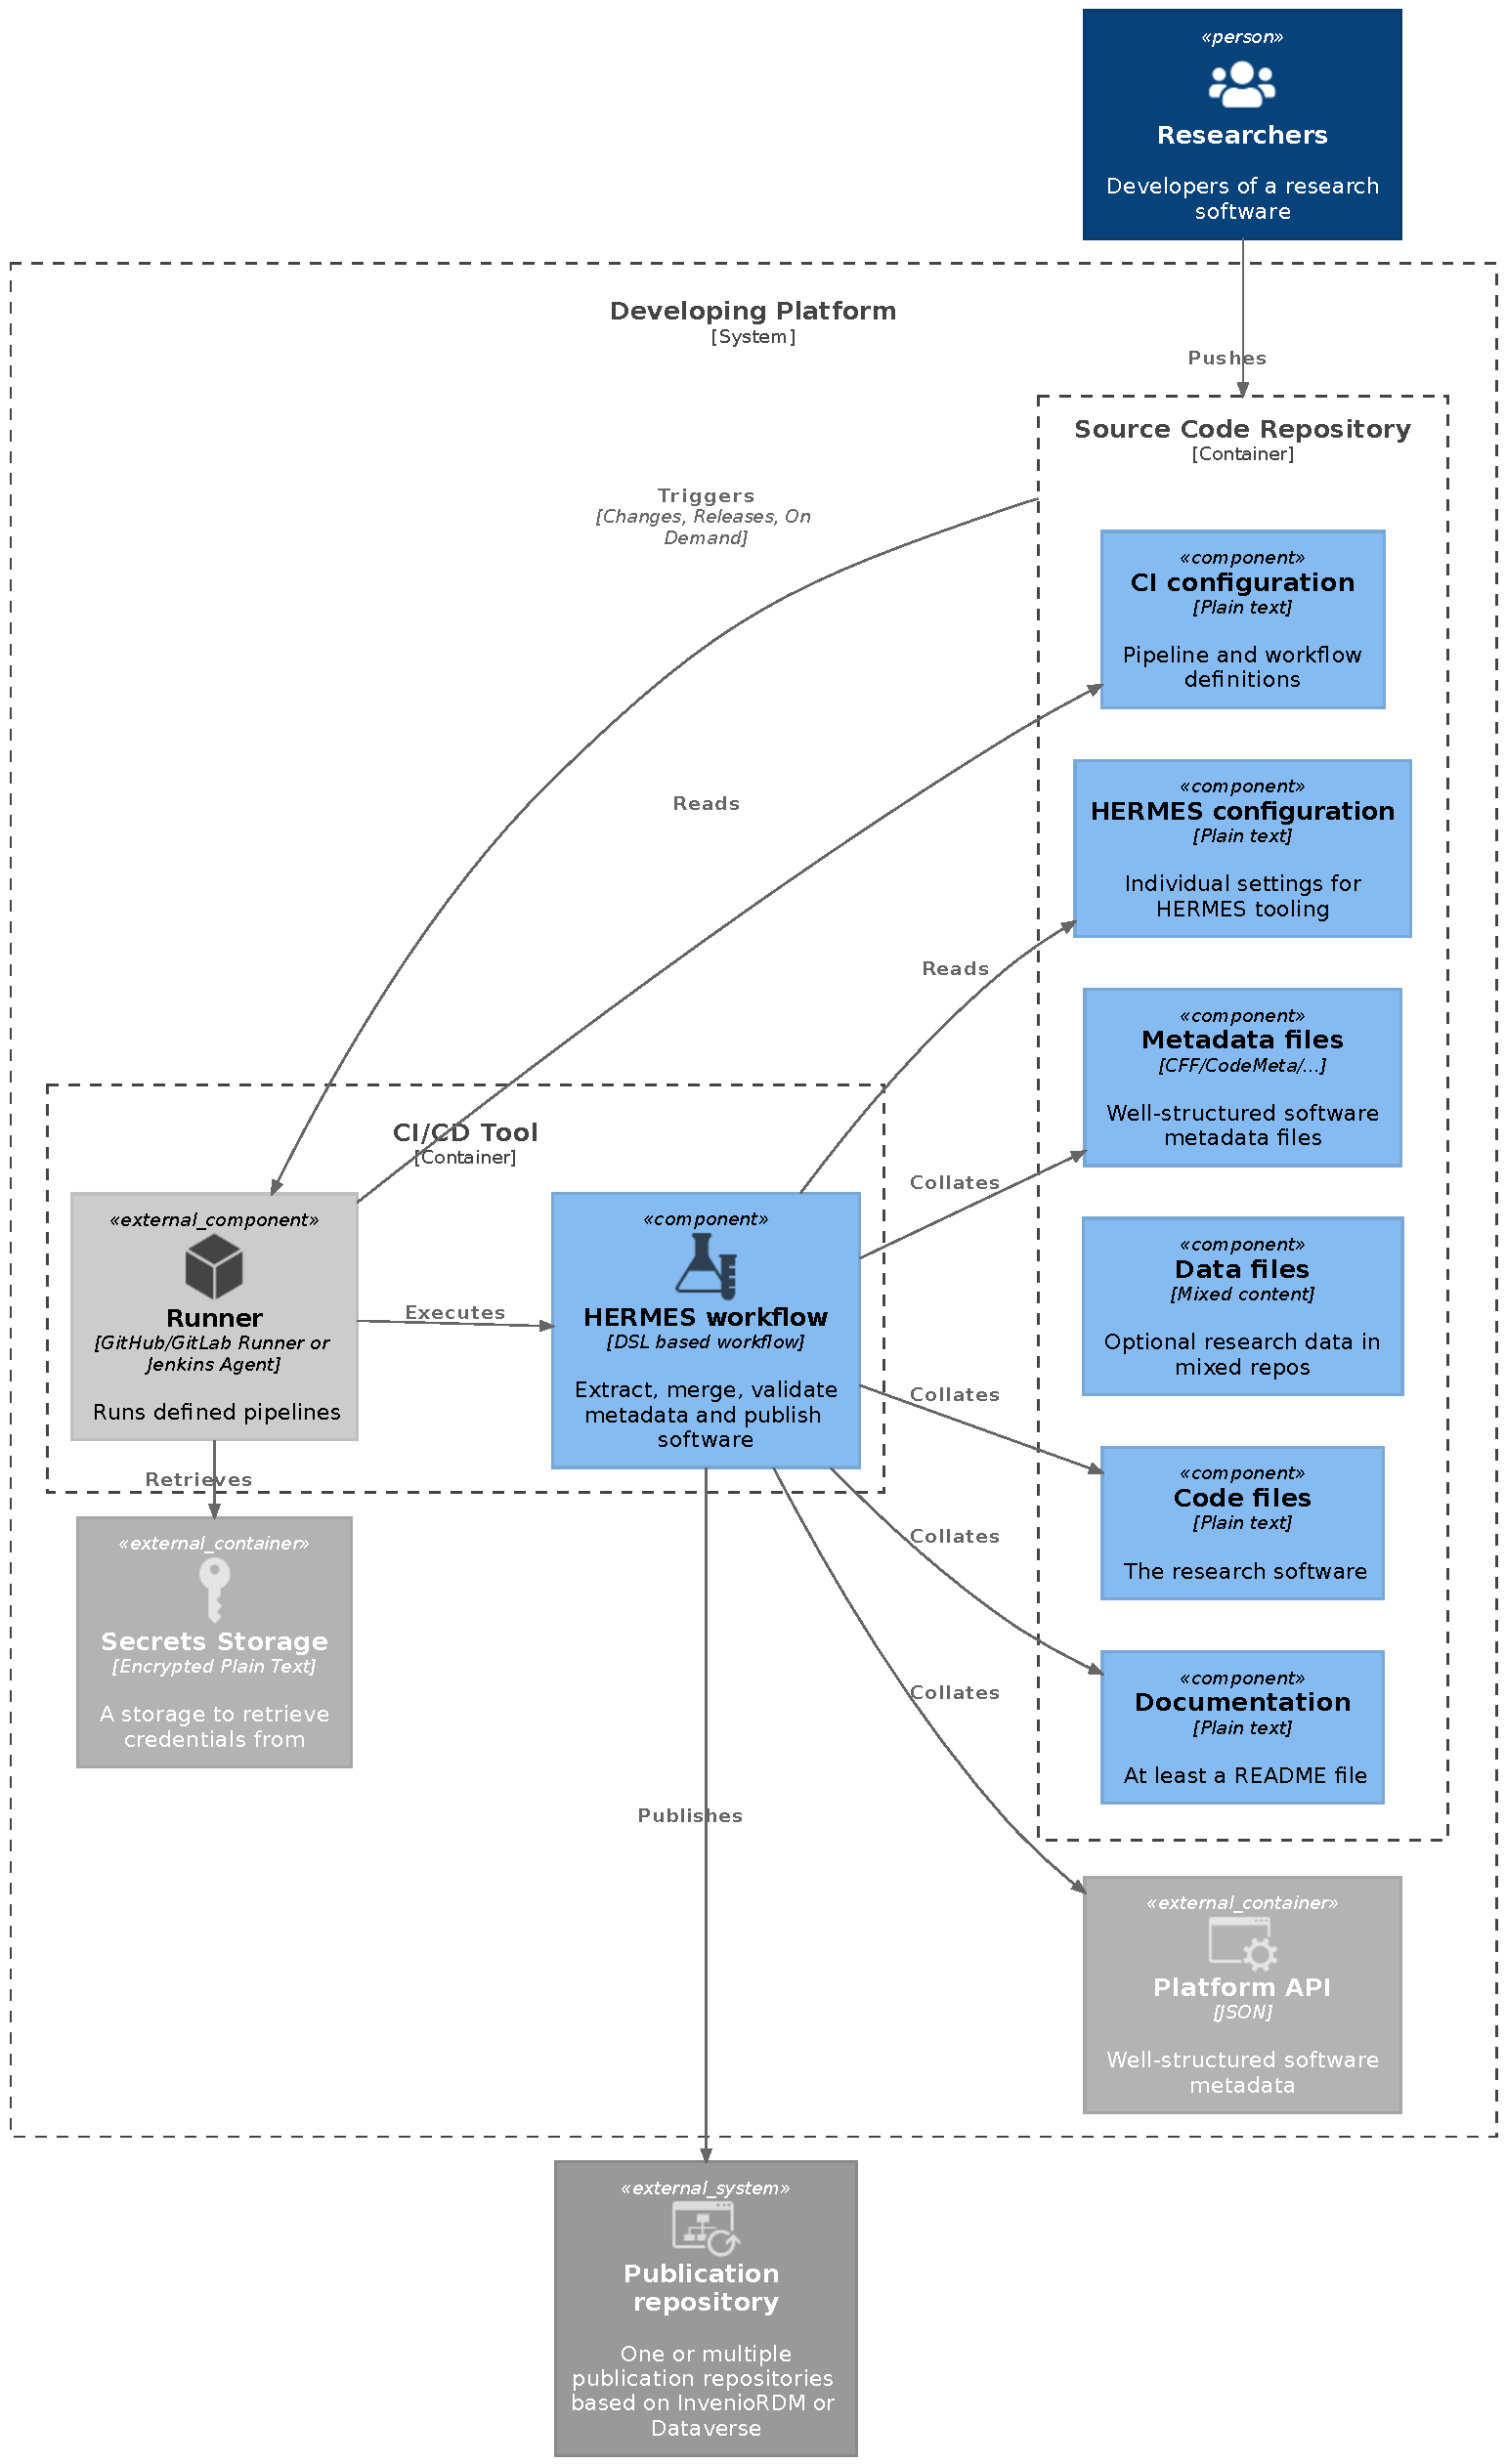
\includegraphics[height=0.9\textheight]{images/architecture/HERMES_System.pdf}
    
    \caption{C4 Component architecture diagram}
    \caption*{Outlining how the HERMES workflow relates to researchers, gets embedded in runners, collates metadata from sources and publishes in target publication repositories.}
    \label{fig:hermes-architecture}
\end{figure}

\begin{figure}[htp]
    \centering
    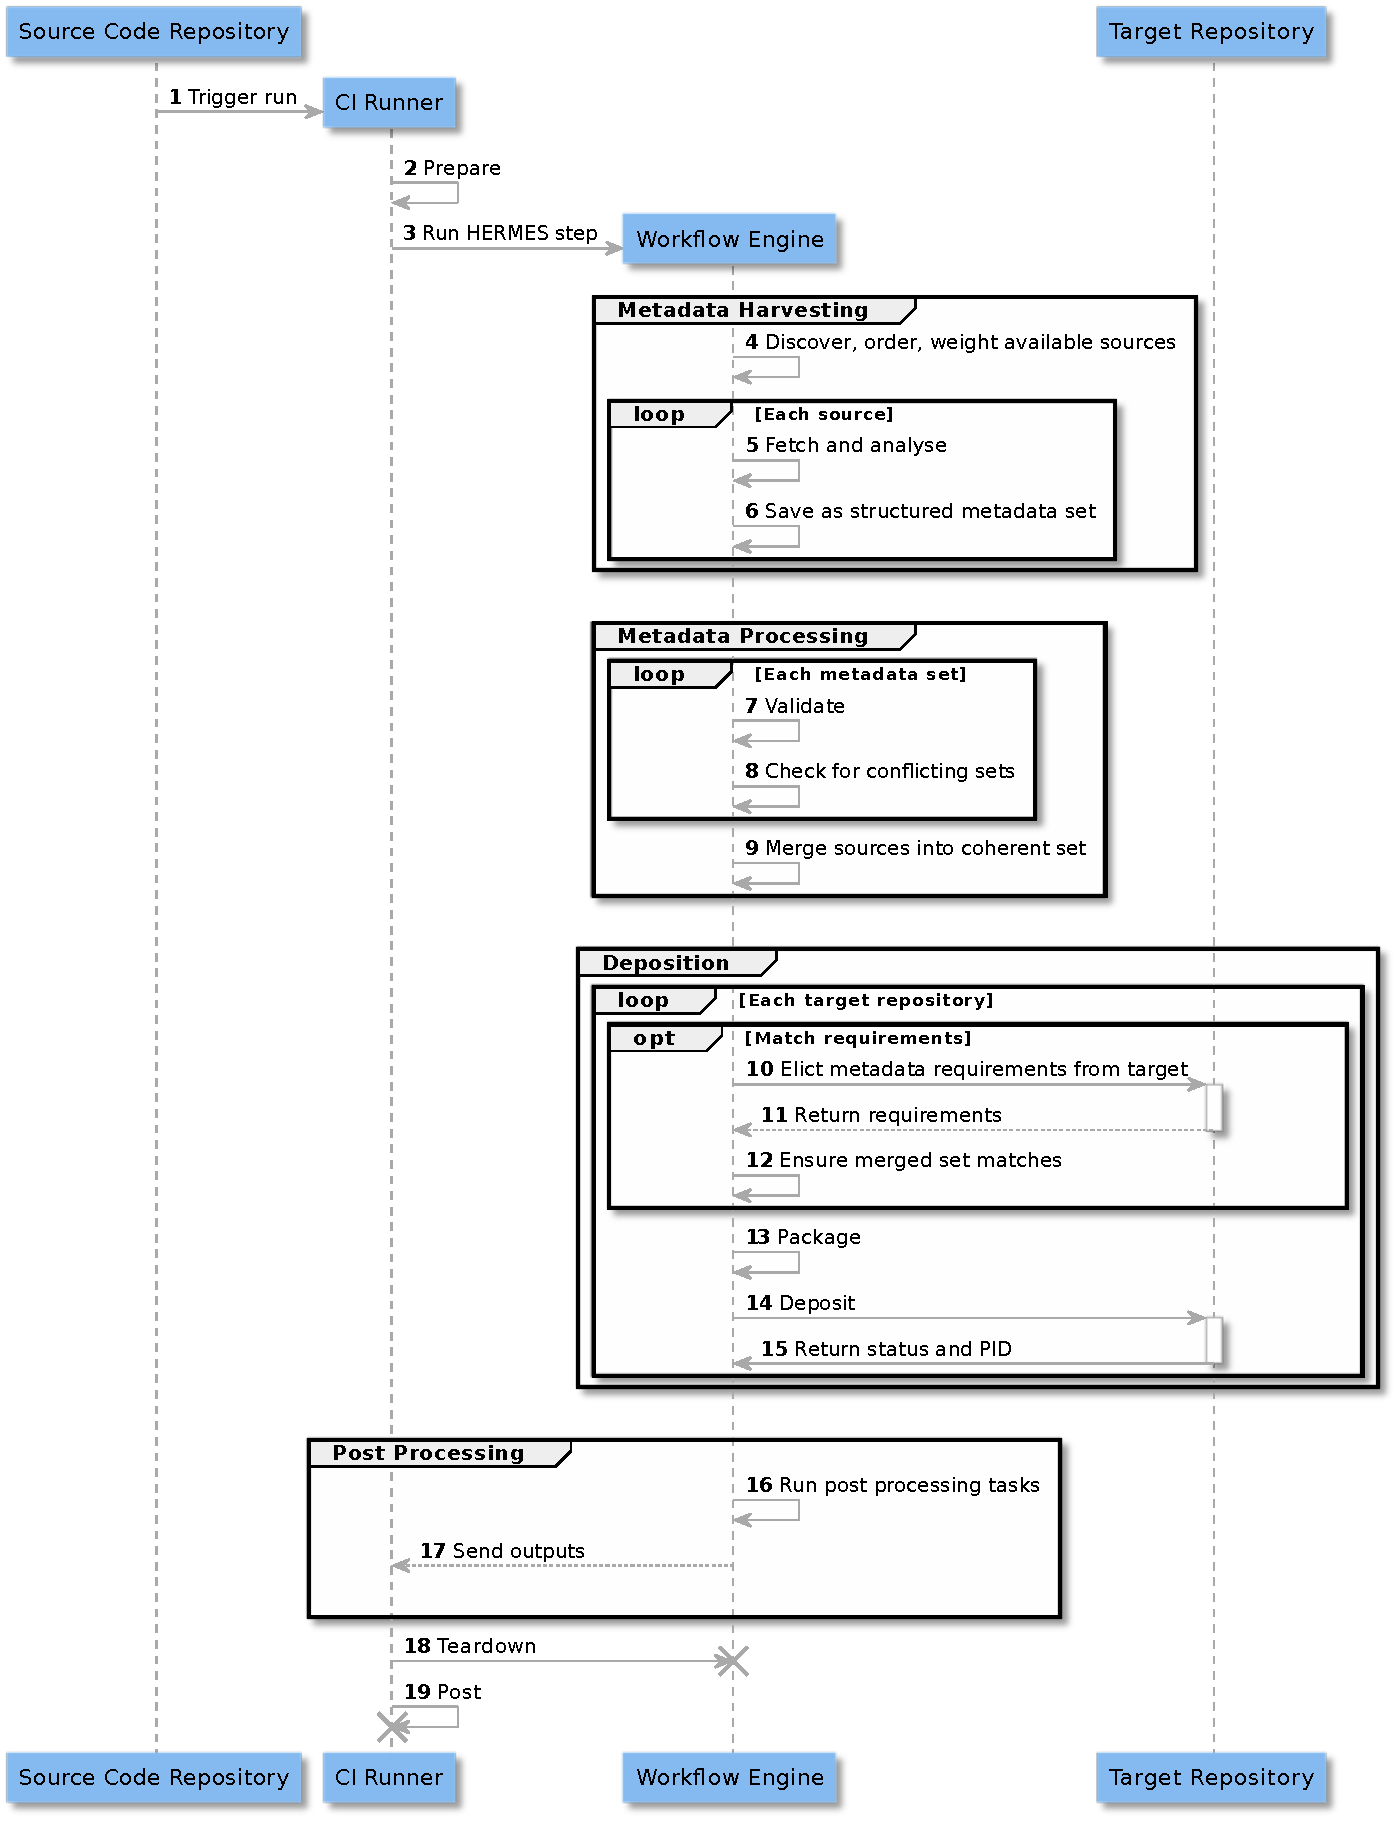
\includegraphics[height=0.85\textheight]{images/workflow/HERMES_Workflow.pdf}
    
    \caption{Sequence diagram of HERMES workflow pipelines}
    \caption*{Simple use case (1 software, n targets) data flow, showing how HERMES workflow pipelines kick into action.
              Outputs of any pipeline are forwarded to the next pipeline. Both \gls{ci-cd} configuration and pipelines
              allow for easy modifications or extensions if necessary.}
    \label{fig:hermes-workflow}
\end{figure}



\clearpage
\addsec{Acknowledgments}\label{acknowledgments}
This project (ZT-I-PF-3-006) was funded by the \enquote{\href{https://www.helmholtz.de/en/about-us/structure-and-governance/initiating-and-networking/}{Initiating and Networking Fund of the Helm\-holtz Association}}
in the framework of the \enquote{\href{https://helmholtz-metadaten.de/en}{Helmholtz Metadata Collaboration}} project call.

We thank the participants of the \href{https://events.hifis.net/event/205/}{project kickoff workshop} for their contributions to the project plan as well as their comments to this document. We especially thank Daniel Garijo (Universidad Politécnica de Madrid), Carlos Martinez-Ortiz (Netherlands eScience Center), Ana Trisovic (Harvard University), Sara Gonzalez (Northwestern University), Dorothea Iglezakis (University Library Stuttgart) and Felix Bach (Karlsruhe Institute of Technology) for presenting their work, as well as Deborah Schmidt (MDC Berlin), Ronny Gey (UFZ Leipzig), Anton Pirogov (FZ Jülich), Dennis Gläser (University of Stuttgart), Jens Bröder (FZ Jülich), Oliver Karras (TIB), Pedro Videgain Barranco (FZ Jülich), Anett Seeland (University of Stuttgart), Kirsten Elger (GFZ German Research Centre for Geosciences) and Jan Göpfert (FZ Jülich).

We highly appreciate the conducted draft paper reviews by Uwe Konrad (HZDR), Bernhard Mittermaier (FZ Jülich), Carina Haupt (DLR) and Ana Trisovic (Harvard University).

We also thank Fonticons, Inc. for free usage of the \href{https://fontawesome.com}{FontAwesome icons} under a \href{https://fontawesome.com/license/free}{CC-BY license} throughout this document.


\setglossarystyle{altlist}
\printglossaries

\phantomsection
\printbibliography[heading=bibintoc]

\end{document}